% vim: set tw=0:
\documentclass{beamer}
\usepackage{graphicx}
\usepackage{hyperref}
\hypersetup{pdfborder={0 0 0 0}}

% Reasonable themes:
% Antibes Bergen Berkeley Berlin Frankfurt Goettingen Ilmenau Luebeck Malmoe
% Montpellier PaloAlto Rochester Singapore Szeged Warsaw bars boxes
% compatibility default lined plain shadow sidebar split tree
% And these ones include the author's name on every slide:
% Berkeley

% Declare themes.
\mode<presentation>
\usetheme{UWHEP}

% Personal macros.
\newcommand{\email}[1]{{\texttt #1}}
\newcommand{\newframe}[1]{\section{#1}
    \frametitle{\sc{#1}}}
\newcommand{\subframe}[1]{\subsection{#1}
    \frametitle{\sc{#1}}}
\newcommand{\supers}[1]{\ensuremath{^\textrm{#1}}}
\newcommand{\subs}[1]{\ensuremath{_\textrm{#1}}}
\newcommand{\ca}{\ensuremath{\sim}}
\renewcommand{\email}[1]{\href{mailto:#1}{\nolinkurl{#1}}}

% Author information.
\title{T2 Status}
\author[Maier, Mohapatra]{
    Will Maier \and Ajit Mohapatra\\
    {\tt wcmaier@hep.wisc.edu}\\
    {\tt ajit@hep.wisc.edu}}
\institute[Wisconsin]{University of Wisconsin - High Energy Physics}
\date{2010.03.30}
\logo{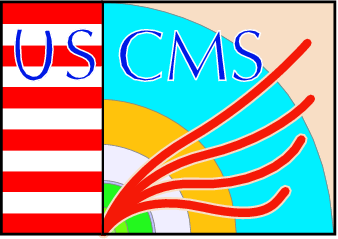
\includegraphics[height=0.6cm]{../../../Graphics/USCMS_logo.png}\hspace{.1cm}
\includegraphics[height=0.75cm]{../../../Graphics/UW_logo.png}}

\begin{document}

\begin{frame}
    \titlepage
\end{frame}

%\section{Overview}
%\begin{frame}
%    \tableofcontents
%\end{frame}

\section{Facilities}
\subsection{Software and Storage}
\begin{frame}
\frametitle{}

\begin{itemize}
	\item 2010.04.06 10:00 - 14:00 CDT: Brief outage to add chilled water backup
	\item 2010.03.28: {\tt dCacheDomain} randomly failed
	\begin{itemize}
		\item No debugging information; increased the JVM heap size and crossed fingers
	\end{itemize}
	\item 2010.03.25: SRM tomcat failed briefly
	\begin{itemize}
		\item Also no debugging information; more heap size bumps and crossed fingers
	\end{itemize}
	\item Wrote a quick interface to aggregate local production data
	\begin{itemize}
		\item Using Python, redis, JS (or matplotlib or gnuplot) for plotting
	\end{itemize}
	\item New storage mostly deployed
	\begin{itemize}
		\item Handling usual glut of early disk failures (data safely replicated by {\tt dcache\_billingrep}
	\end{itemize}
	\item Traffic to Cornell's T3 now prefers NLR over i2
	\begin{itemize}
		\item i2 limited to 200 Mbps at Cornell; NLR is 10Gbps
	\end{itemize}
\end{itemize}
\end{frame}

\subsection{Production and Monitoring}
\begin{frame}
\frametitle{}

\begin{itemize}
	\item JobRobot: OK
	\item SAM: OK
	\item RSV: OK
	\item PhEDEx:
	\begin{itemize}
		\item LoadTest to several clusters of international T2s succeeds and fails on regular 12 and 6 hour intervals
		\item \url{http://savannah.cern.ch/support/?113505}
		\item Still not sure what's wrong; investigating with campus network group, DDT
	\end{itemize}
	\item MC Production:
	\begin{itemize}
		\item 10 TeV production is stopped; only doing 7 TeV
		\item Finishing remaining 7 TeV Alpgens (\ca{}20M) 
		\item Focusing on high priority Minbias (for datataking) production, MC pre-production and redigi/rereco of Summer09 7 TeV samples with CMSSW\_3\_5\_X
	\end{itemize}
\end{itemize}
\end{frame}
\end{document}
